\chapter*{Введение}                         % Заголовок
\addcontentsline{toc}{chapter}{Введение}    % Добавляем его в оглавление

\newcommand{\actuality}{}
\newcommand{\progress}{}
\newcommand{\aim}{{\textbf\aimTXT}}
\newcommand{\tasks}{\textbf{\tasksTXT}}
\newcommand{\novelty}{\textbf{\noveltyTXT}}
\newcommand{\influence}{\textbf{\influenceTXT}}
\newcommand{\methods}{\textbf{\methodsTXT}}
\newcommand{\defpositions}{\textbf{\defpositionsTXT}}
\newcommand{\reliability}{\textbf{\reliabilityTXT}}
\newcommand{\probation}{\textbf{\probationTXT}}
\newcommand{\contribution}{\textbf{\contributionTXT}}
\newcommand{\publications}{\textbf{\publicationsTXT}}

Жидкие кристаллы (ЖК) представляют собой вещества, сочетающие в себе свойства жидкостей и твёрдых тел.
С одной стороны, они способны течь, как вязкие жидкости; с другой стороны, им присуща анизотропия, свойственная кристаллам.
Наиболее исследованными среди них являются нематики, или нематические жидкие кристаллы (НЖК), и холестерики, или холестерические жидкие кристаллы (ХЖК).
Чаще всего молекулы этих веществ имеют вытянутую (стержневидную, конусовидную, каплевидную) форму.
Направление вдоль вытянутой оси молекулы можно обозначить единичным вектором $\textbf{a}$.
Кроме того, существует ещё один класс веществ, у которых наблюдается нематическая или холестерическая упорядоченность.
Это вещества, образованные дискообразными молекулами; в этом случае вектор $\textbf{a}$ направлен также вдоль оси симметрии молекулы.
Усреднение векторов $\textbf{a}$ по физически бесконечно малому объёму после нормировки даёт единичный вектор $\textbf{n}$, называемый директором.
Директор $\textbf{n}$ является важной переменной, позволяющей описывать искажения структуры жидкого кристалла в рамках механики сплошной среды.
Подчеркнём, что в среде выделенной является ось, а не направление, поэтому направления $\textbf{n}$ и $-\textbf{n}$ физически эквивалентны.
При температурах выше некоторой критической ЖК находятся в изотропной фазе, в которой нет выделенного направления, а при температуре ниже критической -- в упорядоченной фазе, в которой директор показывает направление преимущественной ориентации молекул в окрестности данной точки.
Главное отличие НЖК от ХЖК в том, что при температуре ниже критической и в отсутствие внешних воздействий молекулы НЖК выстраиваются вдоль некоторой оси, в то время как молекулы ХЖК образуют так называемую планарную геликоидальную структуру -- периодическую спиральную структуру вдоль некоторого направления в пространстве.
При этом директор $\textbf{n}$ равномерно поворачивается при перемещении вдоль этого направления, оставаясь ему перпендикулярным.
\begin{figure}
	\begin{minipage}{0.49\textwidth}
		\centering
		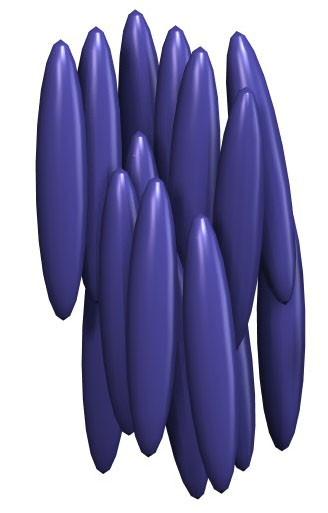
\includegraphics[height=7cm, width=\textwidth]{Nematic_example}
		{А}
	\end{minipage}
	\hfill
	\begin{minipage}{0.49\textwidth}
		\centering
		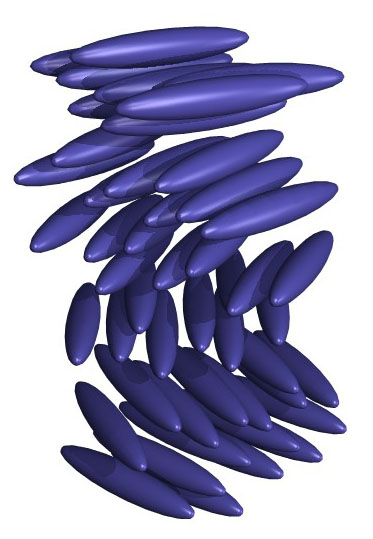
\includegraphics[height=7cm, width=\textwidth]{Cholesteric_example}
		{Б}
	\end{minipage}
	\vspace{0.5cm}
	\caption{Схематическое изображение НЖК (А) и ХЖК (Б)}
\end{figure}

Важной особенностью ЖК является способность к переориентации во внешнем поле, как в магнитном, так и в электрическом.
Это явление, открытое в 1927 году, называется эффектом Фредерикса~\autocite{Fred1927,Fred1933}.
%Примером устройства, в основе работы которого лежит эффект Фредерикса, может служить \todo{TND (twisted nematic device)}
Именно это свойство позволяет использовать ЖК для создания различных электрооптических устройств: систем вывода информации (дисплеев), переключаемых дифракционных решёток, очков и окон с изменяемой светопропускной способностью, беззеркальных лазеров и т.д.~\cite{Blinov1994, McManamon1996, Taheri2000, F.2001, Schmidtke2003, Senyuk2005, Jiang2019}.

Несмотря на то, что эффект Фредерикса изучался в течение долгого времени и для ряда случаев описан как теоретически, так и экспериментально для различных фаз: нематической, холестерической и т.д.~\cite{pikin, deGennesbook1995, stewartBook}, в последнее десятилетие интерес к его изучению возрос~\cite{Brown2003, Brown2007, Makarov2010, Garbovskiy2017, dosSantos2019, Begum2020}.
Большинство исследований идут в сторону усложнения систем и условий, в которых они находятся: рассматриваются различные типы ЖК, геометрии ячеек и граничные условия.
Это в первую очередь связано с возможностью создания систем, обладающих заданными свойствами для потенциальных технических приложений.
При этом наибольший интерес представляют напряжения, индуцирующие переход, а также трансформация равновесной структуры при напряжении выше порогового, так как именно от пространственного распределения директора зависят оптические свойства ячейки.
Важно отметить, что теоретические описания перехода Фредерикса значительно отличаются для магнитного и электрического полей, так как электрическое поле оказывается неоднородным внутри ячейки ЖК~\autocite{Deuling,NonHomoElectricField1972,CTBerr,Arakelyan1984,Napoli2006}.
Ранее переход Фредерикса в нематиках рассматривался как фазовый переход второго рода~\autocite{Guyon1975}, то есть непрерывный фазовый переход.
Однако оказалось, что в киральных нематиках (холестериках) этот переход может быть как непрерывным, так и разрывный, в зависимости от значений материальных констант~\autocite{VAR2013}.

Ещё одно важное свойство ЖК заключается в появлении дополнительной поляризации в результате искажения поля директора.
Такую поляризацию называют \textit{флексоэлектрической}.
%Поляризацию, появляющуюся в ЖК в результате искажения поля директора, называют \textit{флексоэлектрической}.
Первым теоретически описал это явление Майер в 1969 году~\cite{Meyer1969}.
Он дал объяснение~\textit{дипольному} механизму появления флексоэлектрической поляризации для молекул клино- или банановидной формы, обладающих собственным дипольным моментом (см. Рис.~\ref{pic-Meyer}). 

\begin{figure}[ht]
	\centering
	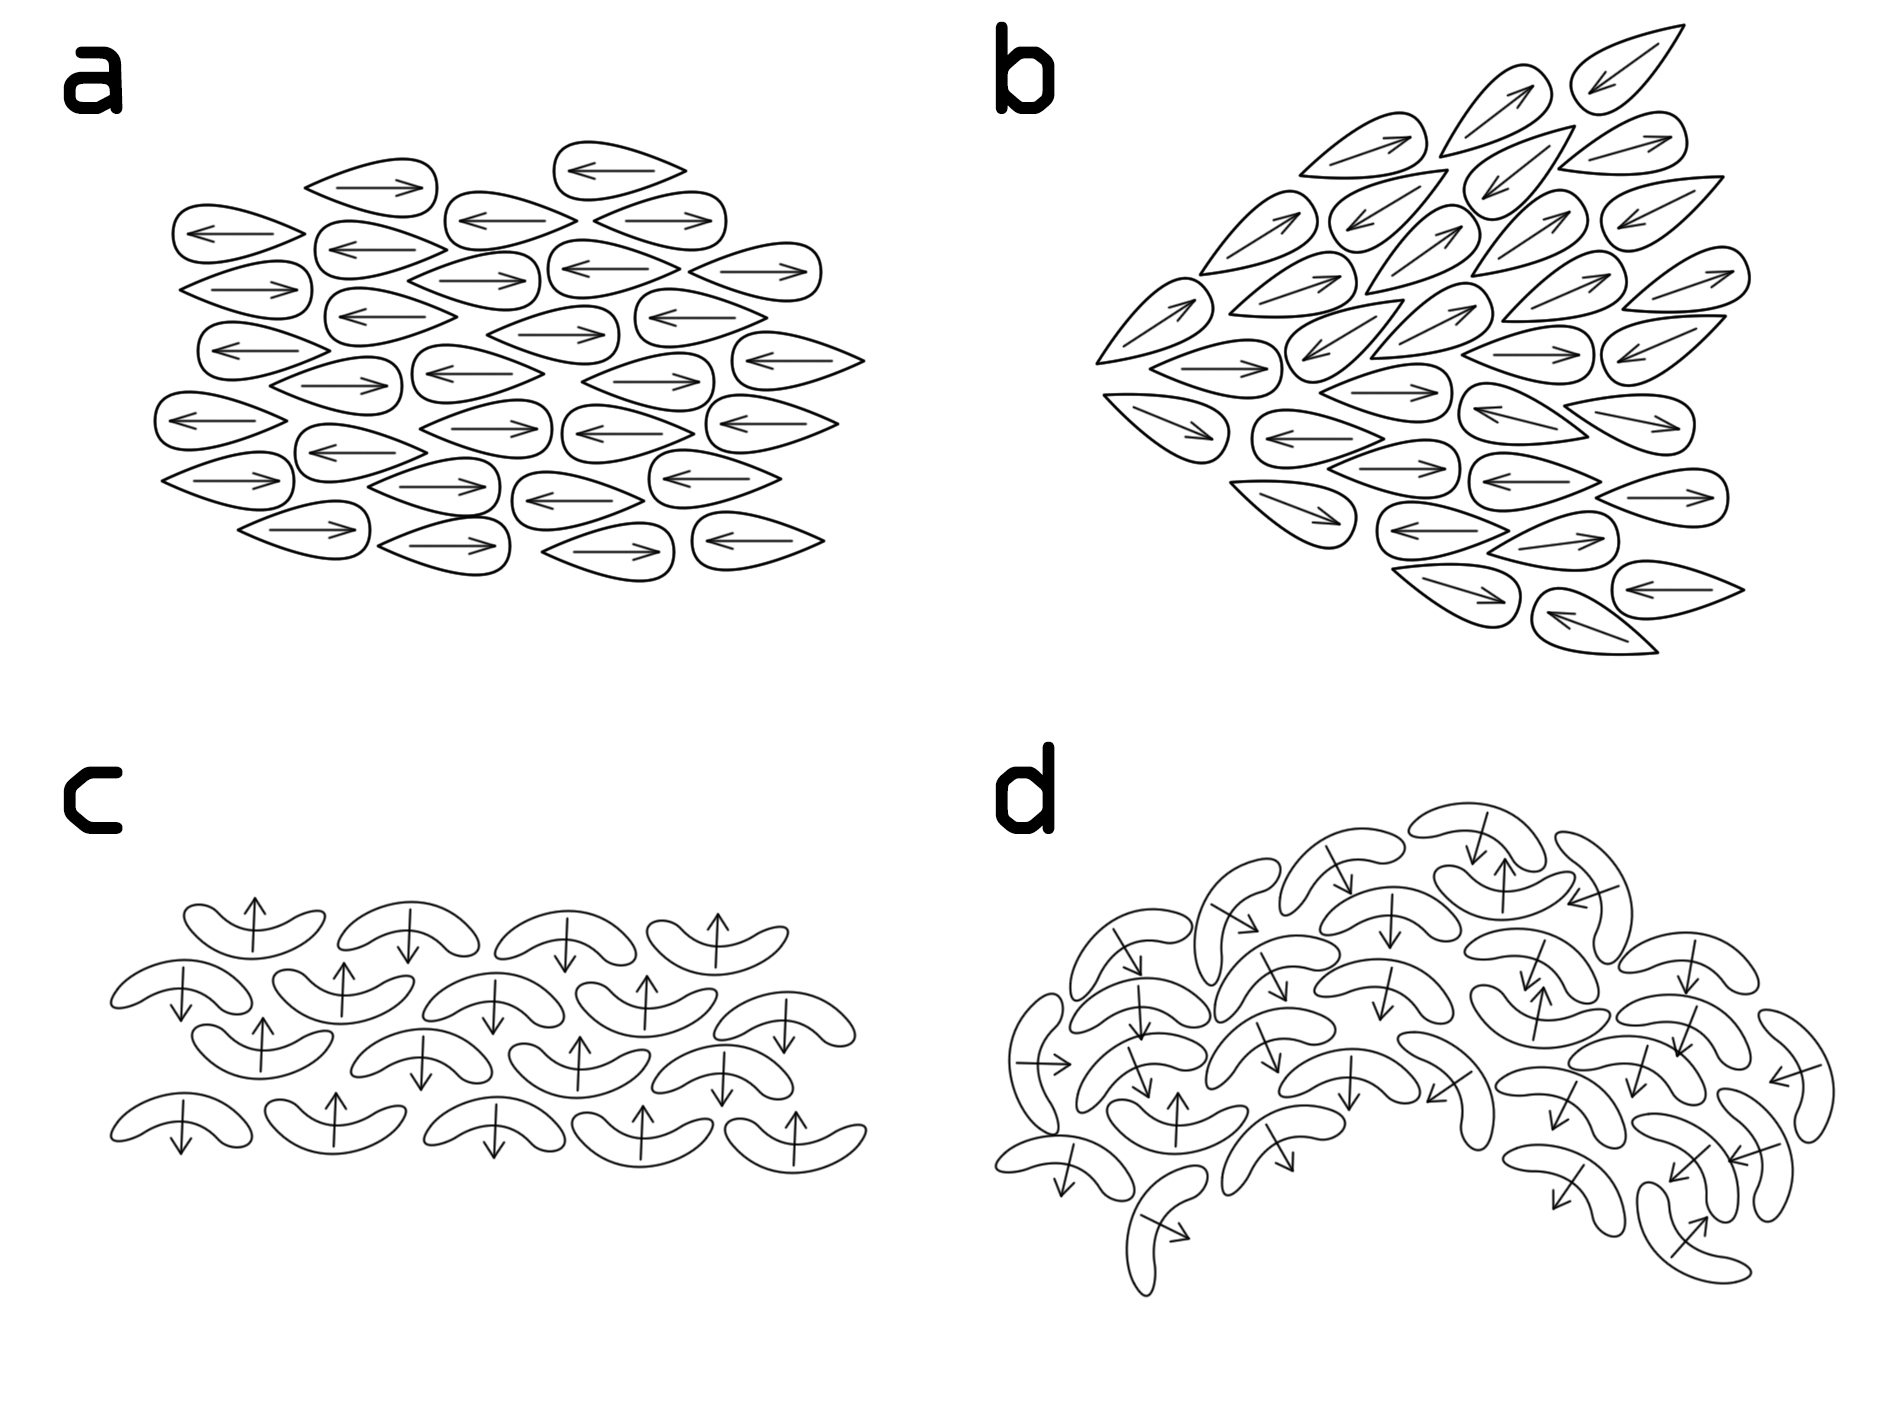
\includegraphics[width=14cm]{Molecules}
	\caption{Появление флексоэлектрической поляризации у молекул специальной формы. Неискажённые состояния для молекул соответственно клиновидной (a) и банановидной (c) формы. Поперечный изгиб, флексоэлектрическая поляризация направлена вправо (b). Продольный изгиб, флексоэлектрическая поляризация направлена вниз (d).}
	\label{pic-Meyer}
\end{figure}

Однако, как показал Прост в 1977 году, этот механизм не является единственным~\cite{Prost77}.
Он объяснил второй известный ныне механизм флексоэлектричества -- квадрупольный.
На рис.~\ref{Prost_explanation}a изображена неискажённая структура из молекул, не обладающих собственным дипольным моментом, но обладающих квадрупольным моментом, причём поляризация в каждом слое равна нулю.
На рис.~\ref{Prost_explanation}b изображена группа таких же молекул, которые подвержены деформации поперечного изгиба.
Видно, что в верхней части области 2 положительный заряд увеличен за счёт квадруполя из области 1.
В то же время, положительный заряд внизу области 2 уменьшился за счёт того, что квадруполи частично перешли в область 3.
Таким образом, данная структура начинает обладать собственным дипольным моментом, направленным вверх, и к ней можно применить всё то, что было сказано про полярные молекулы.
\begin{figure}[ht]
	\centering
	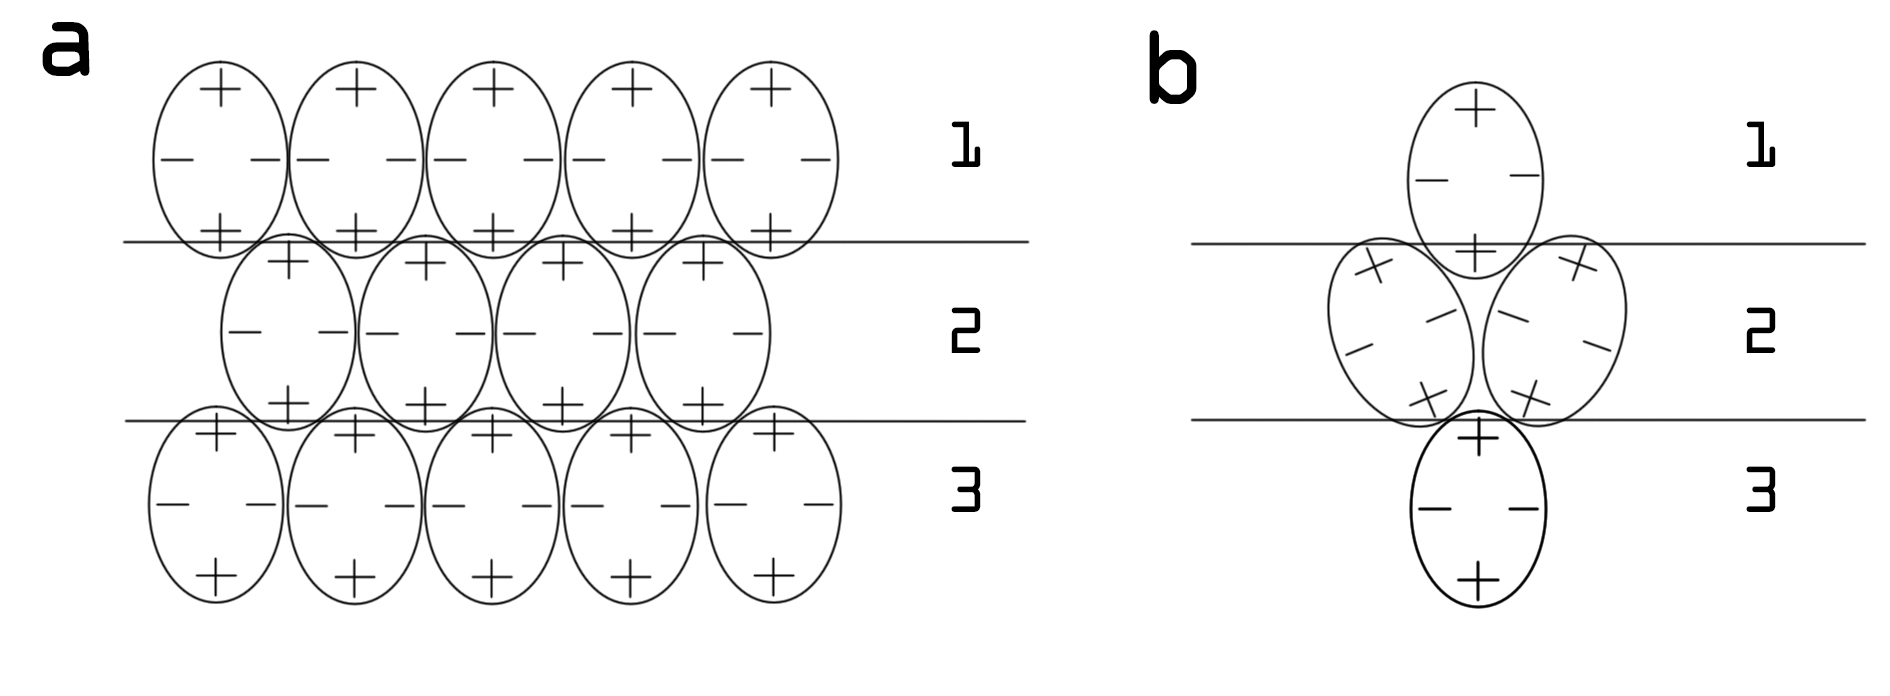
\includegraphics[width=17cm]{Prost_explanation}
	\caption{Симметричные молекулы -- поперечный изгиб}
	\label{Prost_explanation}
\end{figure}

Данная работа посвящена изучению влияния внешнего электрического поля на ориентационную структуру ХЖК с учётом флексоэлектрического эффекта.
Рассматривается ячейка, представляющая собой две проводящие плоскопараллельные пластины, к которым приложено некоторое напряжение; пространство между ними заполнено ХЖК, и ось спирали перпендикулярна ограничивающим плоскостям.
В данной работе исследуется влияние флексоэлектрической поляризации на напряжение, индуцирующее переход Фредерикса в ХЖК при различных параметрах системы, таких как сумма флексоэлектрических коэффициентов,симметричные и несимметричные мягкие граничные условия и др. В первом разделе рассмотрено выражение для свободной энергии ХЖК, отдельно рассмотрен вклад флексоэлектрической поляризации, получены уравнения Эйлера-Лагранжа на равновесную конфигурацию ХЖК, исключён из описания азимутальный угол.
Во втором разделе для случая отрицательной анизотропии диэлектрической проницаемости при помощи численной минимизации функционала свободной энергии найдены равновесные конфигурации при различных условиях.
Также аналитически рассмотрена устойчивость основного состояния ХЖК (планарной геликоидальной структуры).
В третьем разделе аналитически рассмотрен случай, когда вкладом упругой энергии Франка можно пренебречь по сравнению с вкладом, возникающим из-за флексоэлектричества и взаимодействия с электрическим полем, приводится схема возможных трансформаций ориентационной структуры ЖК в зависимости от соотношения материальных параметров системы.
\if 0
\todo{РАЗДЕЛИТЕЛЬ}
Эффект молекулярной переориентации в ячейках жидких кристаллов (ЖК), вызванной внешним полем, широко исследуется, во многом благодаря многообразию приложений.
Это явление, известное как переход (эффект) Фредерикса \textcolor{blue}{был открыт в конце 1920-х годов.(ссылки)}
Среди устройств, в основе работы которых лежит эффект Фредерикса, можно выделить, например, ЖК-дисплеи, переключаемые дифракционные решётки, беззеркальные лазеры и другие~\autocite{YangWu2014}. 
Переход Фредерикса изучался для различных полей: статического электрического и магнитного полей, осциллирующего электрического поля, лазерного излучения, а также для ЖК в различных фазах: нематической, холестерической, смектической и т.~д.~\autocite{Blinov1994,deGennesbook1995,stewartBook}

Простейшим способом учёта взаимодействия с границами является случай жёстких граничных условий.
Слабое зацепление обычно описывается потенциалом Рапини-Папулара~\autocite{Rapini69}.
Важно отметить, что теоретические описания перехода Фредерикса значительно отличаются для магнитного и электрического полей, так как электрическое поле оказывается неоднородным внутри ячейки ЖК~\autocite{Deuling,NonHomoElectricField1972,CTBerr,Arakelyan1984,Napoli2006}.
Ранее переход Фредерикса в нематиках рассматривался как фазовый переход второго рода~\autocite{Guyon1975}, то есть непрерывный фазовый переход.
Однако оказалось, что в киральных нематиках (холестериках) этот переход может быть как непрерывным, так и \todo{разрывный}, в зависимости от материальных констант~\autocite{VAR2013}.

В последнее время наблюдается растёт интерес к изучению влияния флексоэлектричества~\autocite{buka2012flexoelectricity} на пороговые эффекты в ЖК, например, на переключение бистабильных ЖК-устройств~\autocite{Davidson2002,  Parry-Jones2009, Cummings2013}.
Благодарю флексоэлектричеству возникает дополнительное искажение электрического поля, таким образом, оно тоже влияет на переход Фредерикса.
Такой переход в нематических ЖК (НЖК) изучался в работах~\autocite{Brown2003,Brown2007,Mema2017}.
Анализ при этом ограничивался жёсткими граничными условиями, а также приближением низшей гармоники для объёмного распределения директора и электрического поля.

\todo{ДАЛЬШЕ -- ЧТО СДЕЛАНО В РАБОТЕ PRE2018}
Данная работа посвящена теоретическому изучению перехода Фредерикса в случае статического электрического поля в плоскопараллельной ячейке холекстерического ЖК (ХЖК) с учётом флексоэлектрического эффекта, конечной энергии зацепления, а также неоднородности электрического поля внутри ячейки.
При этом задача состоит в нахождении следующих параметров: пороговые напряжения, равновесная конфигурация директора при напряжении выше напряжения перехода \todo{[просто равновесной конфигурации директора?]}, а также род перехода.
Отдельный акцент сделан на устойчивости равновесных структур, а также на построении фазовых диаграмм.

Работа построена следующим образом. В \todo{Секции $N$} выводится выражение для свободной энергии плоскопараллельной ячейки ЖК\todo{, подключённой к источнику}\todo{[, в виде суммы поверхностных и объёмных вкладов]}.
При этом учитывается неоднородность электрического поля внутри ячейки, вызванная диэлектрической анизотропией ЖК и флексоэлектричеством.
Поверхностная свободная энергия описывается потенциалом Рапини-Папулара.
В \todo{Секции $N+1$} находится равновесное распределение директора для широкого спектра материальных констант.
Также при помощи численного вариационного анализа построены фазовые диаграммы, включая зоны стабильности и метастабильности.
В \todo{Секции $N+2$} аналитически изучается устойчивость планарной геликоидальной структуры.
В \todo{Секции $N+3$} исследуется род перехода Фредерикса с использованием двухпараметрической модели Ландау.
В \todo{Секции $N+4$} содержится подведение итогов и обсуждение результатов.
% Счётчик \texttt{citeexternal} используется для подсчёта процитированных публикаций.
\fi
 % Характеристика работы по структуре во введении и в автореферате не отличается (ГОСТ Р 7.0.11, пункты 5.3.1 и 9.2.1), потому её загружаем из одного и того же внешнего файла, предварительно задав форму выделения некоторым параметрам

\textbf{Объем и структура работы.} Диссертация состоит из~введения, трёх глав,
заключения и~двух приложений.
%% на случай ошибок оставляю исходный кусок на месте, закомментированным
%Полный объём диссертации составляет  \ref*{TotPages}~страницу
%с~\totalfigures{}~рисунками и~\totaltables{}~таблицами. Список литературы
%содержит \total{citenum}~наименований.
%
Полный объём диссертации составляет
\formbytotal{TotPages}{страниц}{у}{ы}{}, включая
\formbytotal{totalcount@figure}{рисун}{ок}{ка}{ков} и
\formbytotal{totalcount@table}{таблиц}{у}{ы}{}.   Список литературы содержит
\formbytotal{citenum}{наименован}{ие}{ия}{ий}.
